% Options for packages loaded elsewhere
% Options for packages loaded elsewhere
\PassOptionsToPackage{unicode}{hyperref}
\PassOptionsToPackage{hyphens}{url}
\PassOptionsToPackage{dvipsnames,svgnames,x11names}{xcolor}
%
\documentclass[
  oneside,
  open=any,
  fontsize=11pt]{article}
\usepackage{xcolor}
\usepackage{amsmath,amssymb}
\setcounter{secnumdepth}{-\maxdimen} % remove section numbering
\usepackage{iftex}
\ifPDFTeX
  \usepackage[T1]{fontenc}
  \usepackage[utf8]{inputenc}
  \usepackage{textcomp} % provide euro and other symbols
\else % if luatex or xetex
  \usepackage{unicode-math} % this also loads fontspec
  \defaultfontfeatures{Scale=MatchLowercase}
  \defaultfontfeatures[\rmfamily]{Ligatures=TeX,Scale=1}
\fi
\usepackage{lmodern}
\ifPDFTeX\else
  % xetex/luatex font selection
\fi
% Use upquote if available, for straight quotes in verbatim environments
\IfFileExists{upquote.sty}{\usepackage{upquote}}{}
\IfFileExists{microtype.sty}{% use microtype if available
  \usepackage[]{microtype}
  \UseMicrotypeSet[protrusion]{basicmath} % disable protrusion for tt fonts
}{}
\makeatletter
\@ifundefined{KOMAClassName}{% if non-KOMA class
  \IfFileExists{parskip.sty}{%
    \usepackage{parskip}
  }{% else
    \setlength{\parindent}{0pt}
    \setlength{\parskip}{6pt plus 2pt minus 1pt}}
}{% if KOMA class
  \KOMAoptions{parskip=half}}
\makeatother
% Make \paragraph and \subparagraph free-standing
\makeatletter
\ifx\paragraph\undefined\else
  \let\oldparagraph\paragraph
  \renewcommand{\paragraph}{
    \@ifstar
      \xxxParagraphStar
      \xxxParagraphNoStar
  }
  \newcommand{\xxxParagraphStar}[1]{\oldparagraph*{#1}\mbox{}}
  \newcommand{\xxxParagraphNoStar}[1]{\oldparagraph{#1}\mbox{}}
\fi
\ifx\subparagraph\undefined\else
  \let\oldsubparagraph\subparagraph
  \renewcommand{\subparagraph}{
    \@ifstar
      \xxxSubParagraphStar
      \xxxSubParagraphNoStar
  }
  \newcommand{\xxxSubParagraphStar}[1]{\oldsubparagraph*{#1}\mbox{}}
  \newcommand{\xxxSubParagraphNoStar}[1]{\oldsubparagraph{#1}\mbox{}}
\fi
\makeatother


\usepackage{longtable,booktabs,array}
\usepackage{calc} % for calculating minipage widths
% Correct order of tables after \paragraph or \subparagraph
\usepackage{etoolbox}
\makeatletter
\patchcmd\longtable{\par}{\if@noskipsec\mbox{}\fi\par}{}{}
\makeatother
% Allow footnotes in longtable head/foot
\IfFileExists{footnotehyper.sty}{\usepackage{footnotehyper}}{\usepackage{footnote}}
\makesavenoteenv{longtable}
\usepackage{graphicx}
\makeatletter
\newsavebox\pandoc@box
\newcommand*\pandocbounded[1]{% scales image to fit in text height/width
  \sbox\pandoc@box{#1}%
  \Gscale@div\@tempa{\textheight}{\dimexpr\ht\pandoc@box+\dp\pandoc@box\relax}%
  \Gscale@div\@tempb{\linewidth}{\wd\pandoc@box}%
  \ifdim\@tempb\p@<\@tempa\p@\let\@tempa\@tempb\fi% select the smaller of both
  \ifdim\@tempa\p@<\p@\scalebox{\@tempa}{\usebox\pandoc@box}%
  \else\usebox{\pandoc@box}%
  \fi%
}
% Set default figure placement to htbp
\def\fps@figure{htbp}
\makeatother





\setlength{\emergencystretch}{3em} % prevent overfull lines

\providecommand{\tightlist}{%
  \setlength{\itemsep}{0pt}\setlength{\parskip}{0pt}}



 


\usepackage{booktabs}
\usepackage{longtable}
\usepackage{array}
\usepackage{multirow}
\usepackage{wrapfig}
\usepackage{float}
\usepackage{colortbl}
\usepackage{pdflscape}
\usepackage{tabu}
\usepackage{threeparttable}
\usepackage{threeparttablex}
\usepackage[normalem]{ulem}
\usepackage{makecell}
\usepackage{xcolor}
\usepackage{geometry}
\usepackage{pdflscape}
\usepackage{afterpage}
\usepackage{graphicx}
\usepackage{float}
\usepackage{array}
\usepackage{booktabs}
\usepackage{longtable}
\usepackage{multirow}
\usepackage{wrapfig}
\usepackage{colortbl}
\usepackage{pdflscape}
\usepackage{tabu}
\usepackage{threeparttable}
\usepackage{threeparttablex}
\usepackage[normalem]{ulem}
\usepackage{makecell}
\usepackage{xcolor}
\makeatletter
\@ifpackageloaded{tcolorbox}{}{\usepackage[skins,breakable]{tcolorbox}}
\@ifpackageloaded{fontawesome5}{}{\usepackage{fontawesome5}}
\definecolor{quarto-callout-color}{HTML}{909090}
\definecolor{quarto-callout-note-color}{HTML}{0758E5}
\definecolor{quarto-callout-important-color}{HTML}{CC1914}
\definecolor{quarto-callout-warning-color}{HTML}{EB9113}
\definecolor{quarto-callout-tip-color}{HTML}{00A047}
\definecolor{quarto-callout-caution-color}{HTML}{FC5300}
\definecolor{quarto-callout-color-frame}{HTML}{acacac}
\definecolor{quarto-callout-note-color-frame}{HTML}{4582ec}
\definecolor{quarto-callout-important-color-frame}{HTML}{d9534f}
\definecolor{quarto-callout-warning-color-frame}{HTML}{f0ad4e}
\definecolor{quarto-callout-tip-color-frame}{HTML}{02b875}
\definecolor{quarto-callout-caution-color-frame}{HTML}{fd7e14}
\makeatother
\makeatletter
\@ifpackageloaded{caption}{}{\usepackage{caption}}
\AtBeginDocument{%
\ifdefined\contentsname
  \renewcommand*\contentsname{Table of contents}
\else
  \newcommand\contentsname{Table of contents}
\fi
\ifdefined\listfigurename
  \renewcommand*\listfigurename{List of Figures}
\else
  \newcommand\listfigurename{List of Figures}
\fi
\ifdefined\listtablename
  \renewcommand*\listtablename{List of Tables}
\else
  \newcommand\listtablename{List of Tables}
\fi
\ifdefined\figurename
  \renewcommand*\figurename{Figure}
\else
  \newcommand\figurename{Figure}
\fi
\ifdefined\tablename
  \renewcommand*\tablename{Table}
\else
  \newcommand\tablename{Table}
\fi
}
\@ifpackageloaded{float}{}{\usepackage{float}}
\floatstyle{ruled}
\@ifundefined{c@chapter}{\newfloat{codelisting}{h}{lop}}{\newfloat{codelisting}{h}{lop}[chapter]}
\floatname{codelisting}{Listing}
\newcommand*\listoflistings{\listof{codelisting}{List of Listings}}
\makeatother
\makeatletter
\makeatother
\makeatletter
\@ifpackageloaded{caption}{}{\usepackage{caption}}
\@ifpackageloaded{subcaption}{}{\usepackage{subcaption}}
\makeatother
\usepackage{bookmark}
\IfFileExists{xurl.sty}{\usepackage{xurl}}{} % add URL line breaks if available
\urlstyle{same}
\hypersetup{
  pdftitle={Strategic Resilience and Financial Performance Profile for ESKA BV},
  pdfauthor={Ronald de Boer},
  colorlinks=true,
  linkcolor={blue},
  filecolor={Maroon},
  citecolor={Blue},
  urlcolor={Blue},
  pdfcreator={LaTeX via pandoc}}


\title{Strategic Resilience and Financial Performance Profile for ESKA
BV}
\usepackage{etoolbox}
\makeatletter
\providecommand{\subtitle}[1]{% add subtitle to \maketitle
  \apptocmd{\@title}{\par {\large #1 \par}}{}{}
}
\makeatother
\subtitle{An In-depth Analysis by the Supply Chain Finance Lectoraat,
Hogeschool Windesheim}
\author{Ronald de Boer}
\date{}
\begin{document}
\maketitle


\section{PART 5 - STRATEGIC RESILIENCE
DASHBOARD}\label{part-5---strategic-resilience-dashboard}

\section{PART 5 - STRATEGIC RESILIENCE
DASHBOARD}\label{part-5---strategic-resilience-dashboard-1}

\newgeometry{left=0.8cm,right=0.8cm,top=1.0cm,bottom=0.8cm}
\thispagestyle{empty}

\subsection*{Strategic Supply Chain Resilience
Analysis}\label{strategic-supply-chain-resilience-analysis}
\addcontentsline{toc}{subsection}{Strategic Supply Chain Resilience
Analysis}

\begin{tcolorbox}[enhanced jigsaw, toprule=.15mm, colframe=quarto-callout-note-color-frame, opacityback=0, left=2mm, breakable, arc=.35mm, rightrule=.15mm, bottomrule=.15mm, leftrule=.75mm, colback=white]

\vspace{-3mm}\textbf{\textbf{ESKA BV} - SCRES: \textbf{3.02}/5.00}\vspace{3mm}

\emph{NextGenResilience • RUG • Windesheim • Involvation}

\end{tcolorbox}

\pandocbounded{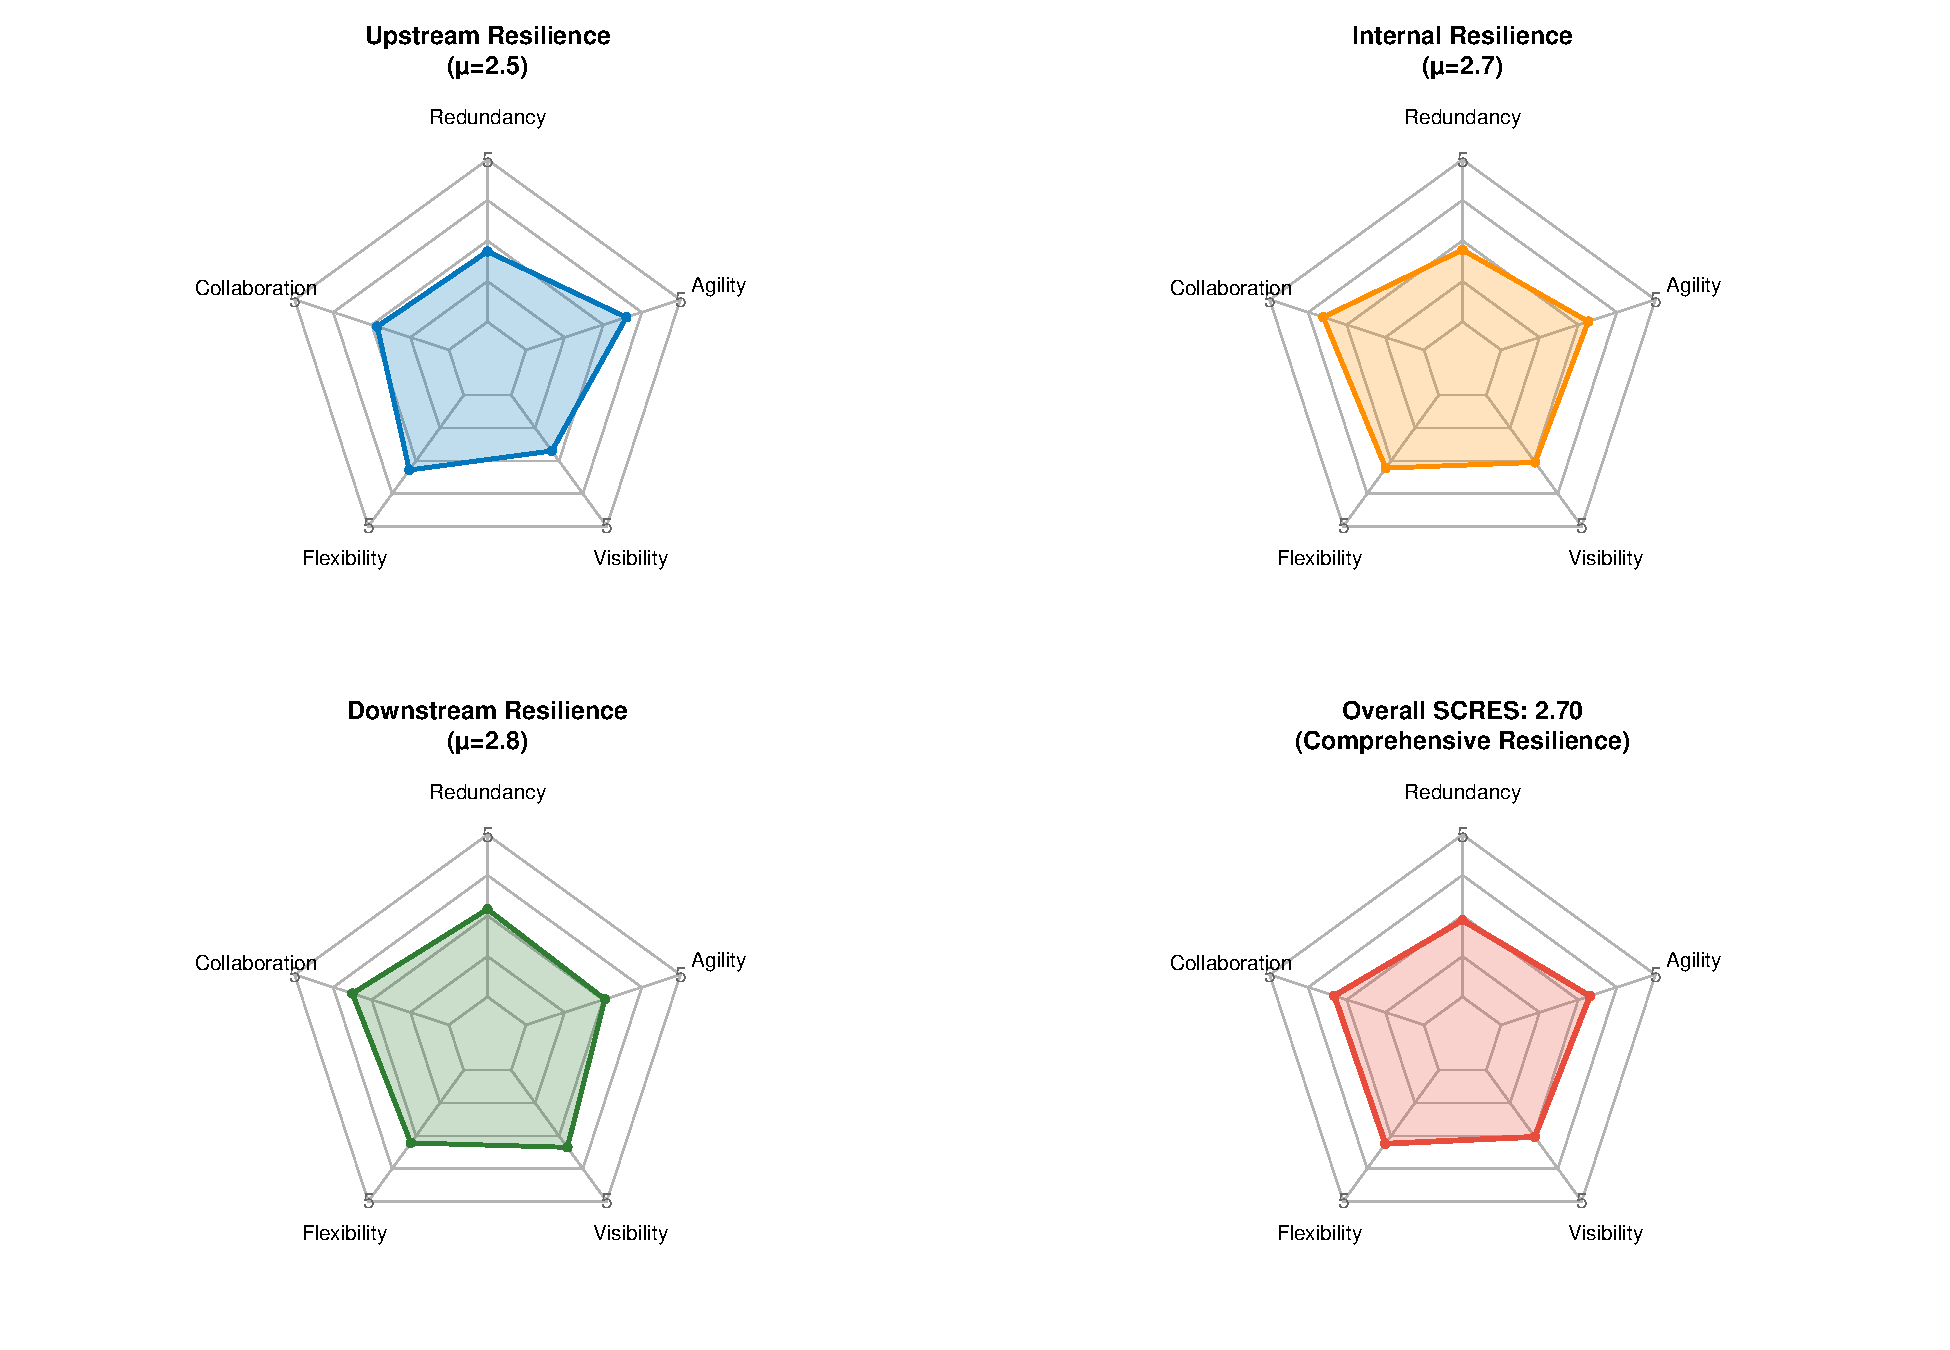
\includegraphics[keepaspectratio]{example_3_files/figure-pdf/main-dashboard-content-1.pdf}}

\begin{tcolorbox}[enhanced jigsaw, toprule=.15mm, colframe=quarto-callout-warning-color-frame, opacityback=0, left=2mm, breakable, arc=.35mm, rightrule=.15mm, bottomrule=.15mm, leftrule=.75mm, colback=white]
\begin{minipage}[t]{5.5mm}
\textcolor{quarto-callout-warning-color}{\faExclamationTriangle}
\end{minipage}%
\begin{minipage}[t]{\textwidth - 5.5mm}

\vspace{-3mm}\textbf{Executive Summary}\vspace{3mm}

\textbf{Performance: Average} (3.02/5.00)

\textbf{Strongest area:} Downstream (3.25)

\textbf{Focus area:} Upstream (2.82)

\end{minipage}%
\end{tcolorbox}

\begin{center}\rule{0.5\linewidth}{0.5pt}\end{center}

\subsection*{Detailed Gap Analysis}\label{detailed-gap-analysis}
\addcontentsline{toc}{subsection}{Detailed Gap Analysis}

\begin{figure}

\begin{minipage}{0.33\linewidth}

\subsubsection{🔵 Upstream}\label{upstream}

\textbf{Gap:} Agility (2.3) vs Redundancy (3.3)\end{minipage}%
%
\begin{minipage}{0.33\linewidth}
\textbf{Hoog:} Multiple suppliers contracted for critical components\\
\textbf{Laag:} Slow response to supplier disruptions\end{minipage}%
%
\begin{minipage}{0.33\linewidth}

\subsubsection{🟡 Internal}\label{internal}

\textbf{Gap:} Flexibility (2.5) vs Collaboration (3.9)\end{minipage}%
\newline
\begin{minipage}{0.33\linewidth}
\textbf{Hoog:} Weekly planning sessions with key suppliers\\
\textbf{Laag:} Rigid contract terms without flexibility\end{minipage}%
%
\begin{minipage}{0.33\linewidth}

\subsubsection{🟢 Downstream}\label{downstream}

\textbf{Gap:} Visibility (2.5) vs Redundancy (3.6)\end{minipage}%
%
\begin{minipage}{0.33\linewidth}
\textbf{Hoog:} Multiple suppliers contracted for critical components\\
\textbf{Laag:} Limited insight into supplier processes\end{minipage}%

\end{figure}%

\restoregeometry




\end{document}
